\documentclass[tikz,border=8pt]{standalone}
\usepackage{tikz}
\usepackage{tkz-euclide}
\usepackage{amsmath, amssymb}

\usetikzlibrary{angles, quotes}

\begin{document}

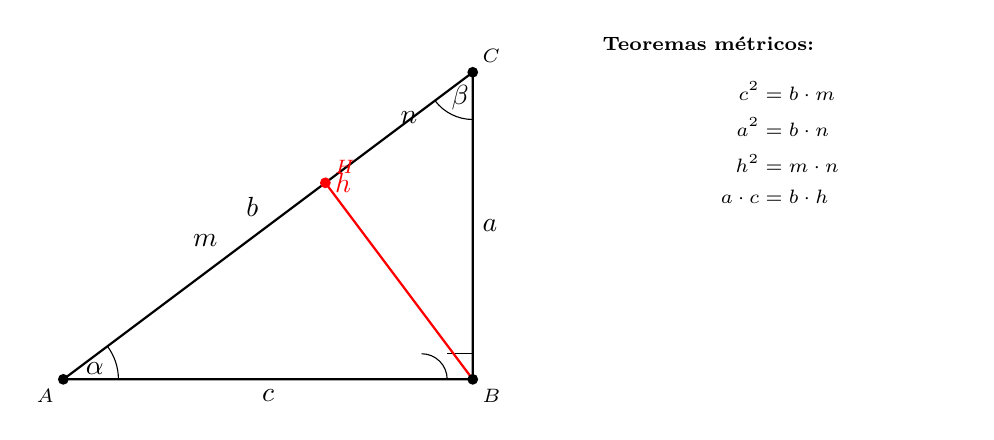
\begin{tikzpicture}[scale=1.3]

  % ---- Triángulo rectángulo ABC recto en B ----
  \coordinate (A) at (0,0);
  \coordinate (B) at (4,0);
  \coordinate (C) at (4,3);

  \draw[thick] (A) -- (B) -- (C) -- cycle;

  % ---- Ángulo recto en B ----
  \draw (3.75,0) arc (0:90:0.25);
  \draw (3.75,0.25) -- (4,0.25) -- (4,0);

  % ---- Altura relativa a la hipotenusa BH ----
  \coordinate (H) at ({4*(16/25)},{4*(12/25)});  % pie de la altura
  \draw[red, thick] (B) -- (H);

  % ---- Proyecciones sobre la hipotenusa: AH = m, HC = n ----
  % Hipotenusa AC va de (0,0) a (4,3)
  % Proyección de cateto AB sobre AC: m = c^2/b = 16/5 = 3.2
  % Proyección de cateto BC sobre AC: n = a^2/b = 9/5 = 1.8
  \coordinate (m_end) at ({3.2*(4/5)},{3.2*(3/5)});  % punto a distancia m desde A
  \coordinate (n_end) at ({4},{3});  % C

  % Etiquetas de proyecciones
  \node[above left] at (1.6,1.2) {$m$};
  \node[above right] at (3.2,2.4) {$n$};

  % ---- Etiquetas de lados ----
  \node[below] at (2,0) {$c$};
  \node[right] at (4,1.5) {$a$};
  \node[above left] at (2,1.5) {$b$};

  % ---- Etiqueta de altura ----
  \node[red, right] at (H) {$h$};

  % ---- Vértices ----
  \fill (A) circle (1.5pt) node[below left] {\scriptsize $A$};
  \fill (B) circle (1.5pt) node[below right] {\scriptsize $B$};
  \fill (C) circle (1.5pt) node[above right] {\scriptsize $C$};
  \fill[red] (H) circle (1.5pt) node[above right] {\scriptsize $H$};

  % ---- Ángulos para identificar ----
  \pic["$\alpha$", draw, angle radius=0.7cm] {angle=B--A--C};
  \pic["$\beta$", draw, angle radius=0.6cm] {angle=A--C--B};

  % ---- Compendio de teoremas (texto pequeño dentro de la figura) ----
  \node[align=left, text width=4.5cm, font=\scriptsize] at (7, 2.5) {
    \textbf{Teoremas métricos:}
    \begin{align*}
      c^2 &= b \cdot m \\
      a^2 &= b \cdot n \\
      h^2 &= m \cdot n \\
      a \cdot c &= b \cdot h
    \end{align*}
  };

\end{tikzpicture}

\end{document}
